% 2019-02-06

\documentclass[10pt]{article}
\usepackage[T1]{fontenc}
\usepackage{amssymb}
\usepackage{amsmath}
\usepackage{graphicx}
% \begin{figure}[h]
% \centering
% \includegraphics[width=6.5in]{folder/photo.png}
% \caption{}
% \label{}
% \end{figure}



\usepackage{tikz}
\usetikzlibrary{arrows}
\usepackage{subfigure}
\usepackage{stackrel}
\usepackage{blindtext}

\usepackage[url=false]{biblatex}
\addbibresource{library.bib}

\oddsidemargin=0.15in
\evensidemargin=0.15in
\topmargin=-.5in
\textheight=9in
\textwidth=6.25in

\usepackage[colorlinks=true,breaklinks,pdfpagemode=none,linkcolor=blue,citecolor=blue]{hyperref}

\usepackage{enumerate}
% \vspace{-6pt}
% \begin{itemize}
%     \setlength{\itemsep}{0pt}%
%     \setlength{\parskip}{0pt}%
%     \item Item 1
%     \item Item 2
%         \begin{itemize}
%             \setlength{\itemsep}{0pt}%
%             \setlength{\parskip}{0pt}%
%             \item Sublist Item 1
%             \item Sublist Item 2
%         \end{itemize}
%         \item Item 3
% \end{itemize}
% \vspace{-6pt}


\usepackage{enumitem}
\setlist{itemsep=0mm}

\usepackage{amsmath,amsfonts,amssymb,bm}



\begin{document}

   \noindent
   \begin{center}

   \hrulefill
   
   \vspace{5pt}
   
   \makebox[\textwidth]{ {\bf Energy Systems Analysis} \hfill  A.D. Smith 2019}
   \vspace{0pt}
   
   {\Large \hfill  Lecture 12. BEM: Building Systems, Part I\\ \hfill {\large Envelope, Zones, Interior}}
   \vspace{5pt}
   
  
   \hrulefill
   \end{center}

{\center{ \small{      ``Commercial buildings are complicated thermodynamic objects.''
\\%[3pt]
\rightline{{\rm --- Samuelson, Ghorayshi, and Reinhart \cite{Samuelson2016-ml}}}}}}



\section{Envelope and Construction}

The building envelope, or ``skin'' of the building, protects the building and its occupants from the elements and from a control-volume, single-building perspective, it defines your system boundary for the building. 

The building's construction, including the envelope as well as interior walls and structures, can be specified to EnergyPlus as \cite{EPcourseteaching}:

\vspace{-6pt}
\begin{itemize}
    \setlength{\itemsep}{0pt}%
    \setlength{\parskip}{0pt}%
    \item Surfaces grouped into zones
    \item Individual structures like:
        \begin{itemize}
            \setlength{\itemsep}{0pt}%
            \setlength{\parskip}{0pt}%
            \item Walls
            \item Roofs
            \item Ceilings
            \item Floors
        \end{itemize}
        \item Individual materials
        \item Groups of materials, called Constructions or Construction Sets in EnergyPlus-speak.
\end{itemize}
\vspace{-6pt}

As an EnergyPlus building simulation comes together, information from the IDF, organized according to the IDD, will be expected by EnergyPlus to fall into a hierarchy of data for processing. The hierarchy for the building's envelope is shown in Figure \ref{hierarchy}.

\begin{figure}[h]
\centering
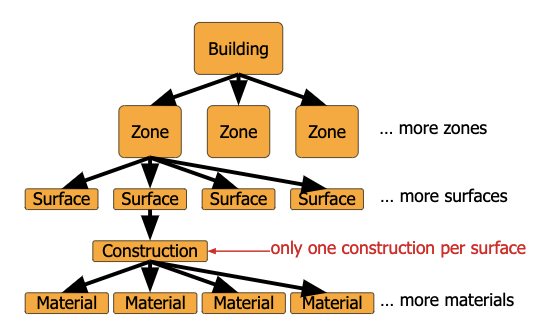
\includegraphics[width=4.5in]{extras12/envelopehierarchy.png}
\caption{Envelope Hierarchy in EnergyPlus \cite{EPcourseteaching}}
\label{hierarchy}
\end{figure}

It is a best practice to use ``as few surfaces as necessary'' \cite{EPcourseteaching}, meaning that you define a construction or surface and reuse for multiple walls if possible. This will require knowledge of the materials and methods used for construction, and an understanding of important phenomena at the interface of building constructions (like thermal bridging; see Lecture 8).

\section{Thermal Zoning}

Remember that the thermal zones, simply called Zones in EnergyPlus-speak, are not geometric entities but rather groups of things that will interact thermally. According to the Getting Started documentation:

\begin{quote}
    The \textbf{thermal zone} is defined as a volume of air at a uniform temperature. \cite{EPdocs9gettingstarted}
\end{quote} 

This leads to one general rule: 

\begin{quote}
Use the number of fan systems (and radiant systems) not the number of rooms to determine the
number of zones in the building. \cite{EPdocs9gettingstarted}
\end{quote}

It is best practice in any case to use ``as few zones as necessary'' \cite{EPcourseteaching}, meaning that you have just enough zones to adequately capture the phenomena that will help you make decisions based on model output, but no more zones which would add to model complexity or computational time (or likely both).\\

The rule above can be expanded toward a more systems thinking-type view of the buiding:

\begin{quote}
    The minimum number of zones in a general simulation model will
usually be equal to the number of systems serving the building. The collection of heat transfer and
heat storage surfaces defined within each zone will include all surfaces bounding or inside of the
space conditioned by the system.
\end{quote}

Making zoning decisions beyond these guidelines will require deep engineering knowledge about the interactions between building constructions, mechanical systems, occupants, and the thermal masses within the building as a whole. Furthermore, the exact same building might actually need more zones for a model that requires greater differentiation in thermal conditions within the building than it would for another, more general, model. The key is to understand how the information produced by the model will be used.

\section{Interior Environment}

\subsection{Internal Gains and People}

People in a building are referred to as \textbf{occupants} in the world of building science. People are a type of \textbf{internal gain}, meaning that they add heat to the building's interior. For example, our skin can dissipate latent heat through sweating (evaporation) and sensible heat by convection or radiation.

\begin{description}
\item[Sensible heat] energy addition associated with (dry-bulb) temperature change in zone \cite{EPcourseteaching}
\item[Latent heat] energy addition associated with moisture/humidity change in zone \cite{EPcourseteaching} 
\end{description}

There are three major categories of drivers for \textbf{sensible heat gains} typically seen in buildings \cite{EPcourseteaching}:


\begin{description}

\item[Convection] ``instantaneous additions of heat to the zone air'' \cite{EPdocs9engineering}
\item[Thermal (long wave) radiation]
\item[Visible (short wave) radiation]
\end{description}


When heat is added to the interior spaces via radiation, ``Radiant gains
are distributed on the surfaces of the zone, where they are first absorbed and then released back
into the room (with some fraction conducted through the surface) according to the surface heat
balances.'' \cite{EPdocs9engineering} 

When there is \textbf{latent heat gain} in the interior spaces because of evaporation, ``Latent gains must
be handled by ventilation or air conditioning equipment.'' \cite{EPdocs9engineering}

There are a few different ways we can provide information about the number of people in a zone \cite{EPdocs9inputoutput}:
\vspace{-6pt}
\begin{itemize}
    \setlength{\itemsep}{0pt}%
    \setlength{\parskip}{0pt}%
\item Number of People [person]
\item People per Zone Floor Area [person/$m^2$]
\item Zone Floor Area per Person [$m^2$/person]
\end{itemize}


We will also need to provide some additional information to help EnergyPlus know how to deal with the people as it implements energy and mass balances. A few key fields are shown here, but the full set of options and their default values, where applicable, can be found in the Input-Output Reference \cite{EPdocs9inputoutput}.

\begin{itemize}
    \setlength{\itemsep}{0pt}%
    \setlength{\parskip}{0pt}%
\item Fraction Radiant [unitless, 0 to 1]---``used to characterize the type of heat being
given off by people in a zone \ldots The remainder of the sensible load is assumed to be convective heat gain. Note that latent gains
from people are not included in either the radiant or convective heat gains.'' \cite{EPdocs9inputoutput}
\item Carbon Dioxide Generation Rate [$m^3$/(s-W)]
\item Clothing Insulation Calculation Method [key/choice field]---``tells which of the next two fields are filled and is descriptive of the
method for calculating the clothing insulation value of occupants.'' \cite{EPdocs9inputoutput}
\end{itemize}
\vspace{-6pt}


\subsection{Lighting}

Lighting is a type of internal gain, notably radiant in the visible region (short wave radiation). However, lights will transfer even more radiant energy in the form of thermal (long wave) radiation \cite{EPdocs9engineering}. The visible radiant gain will be a larger fraction compared with the thermal radiant gain for energy efficient lighting fixtures.

We use a Lights statement to provide information to EnergyPlus about lighting at the zone level. ``A zone may have multiple Lights statements. For example, one statement may describe the general
lighting in the zone and another the task lighting. Or you can use multiple Lights statements for a zone
that has two or more general lighting systems that differ in design level, schedule, etc.'' \cite{EPdocs9inputoutput} A few key fields are shown here, but the full set of options and their default values, where applicable, can be found in the Input-Output Reference \cite{EPdocs9inputoutput}.

\begin{itemize}
    \setlength{\itemsep}{0pt}%
    \setlength{\parskip}{0pt}%
\item Design Level Calculation Method [key/choice field]---``tells which of the next three fields are filled and is descriptive of
the method for calculating the nominal lighting level in the Zone.'' \cite{EPdocs9inputoutput}
\begin{itemize}
    \setlength{\itemsep}{0pt}%
    \setlength{\parskip}{0pt}%
    \item LightingLevel [W]
    \item Watts/Area [W/$m^2$]
    \item Watts/Person [W/person]
\end{itemize}
\item Fraction Visible [unitless, 0 to 1]
\item Return Air Fraction [unitless, 0 to 1]---``fraction of the heat from lights that goes into the zone return air'' \cite{EPdocs9inputoutput}
\end{itemize}
\vspace{-6pt}


% Electric lights full-on assumed to provide the setpoint illuminance – regardless of schedule
% Electric lighting control system simulated to determine fraction of lighting for each lighting zone
% Based on daylighting illuminance level regardless of actual electric lighting input power
% Zone lighting electric reduction factor passed to thermal calculation
% Heat gain from lights and power input reduced



\subsection{Equipment}

Equipment is a type of internal gain, often  radiant in the form of thermal (long wave) radiation. We could technically include lighting as a type of equipment, but since lighting is its own end-use category, often evaluated separately from the equipment types shown here, EnergyPlus groups non-lighting related equipment together.

\subsubsection{Electric equipment}

Electric equipment encompasses ``plug loads'' such as computers, TVs, microwaves, or anything else the occupants have plugged in. Similarly to lighting, above, a few key fields are shown here, and the full set of options and their default values, where applicable, can be found in the Input-Output Reference \cite{EPdocs9inputoutput}.

\begin{itemize}
    \setlength{\itemsep}{0pt}%
    \setlength{\parskip}{0pt}%
\item Design Level Calculation Method [key/choice field]---``tells which of the next three fields are filled and is descriptive of
the method for calculating the nominal electric equipment level in the Zone.'' \cite{EPdocs9inputoutput}

\begin{itemize}
    \setlength{\itemsep}{0pt}%
    \setlength{\parskip}{0pt}%
    \item EquipmentLevel [W]
    \item Watts/Area [W/$m^2$]
    \item Watts/Person [W/person]
\end{itemize}
\item Heat Gains from Electric Equipment 
\begin{itemize}
    \setlength{\itemsep}{0pt}%
    \setlength{\parskip}{0pt}%
    \item Fraction Latent [unitless, 0 to 1]
    \item Fraction Radiant [unitless, 0 to 1]
    \item Fraction Lost [unitless, 0 to 1]---e.g. ``electrical energy converted to mechanical
work or heat that is vented to the atmosphere.'' \cite{EPdocs9inputoutput}
\end{itemize}

\end{itemize}
\vspace{-6pt}


\subsubsection{Other equipment}

Other equipment types in EnergyPlus that have same input format as Electric Equipment (just a different keyword):

\begin{itemize}
    \setlength{\itemsep}{0pt}%
    \setlength{\parskip}{0pt}%
    \item Gas Equipment
    \item Hot Water Equipment
    \item Steam Equipment
    \item Other Equipment (``provided as an additional source for heat gains or losses directly to the zone
with a fuel type that is configurable.'' \cite{EPdocs9inputoutput})
\end{itemize}



\subsection{Schedules}

Schedules describe \textit{when} things happen in the simulated building, e.g. occupancy density, illumination, thermostats, and more.

Internal gains can be ``described to EnergyPlus as a design or peak level with a
schedule that specifies a fraction of the peak for each hour'' \cite{EPdocs9gettingstarted}. EnergyPlus uses a nested set of schedule pieces to build unique schedules \cite{EPcourseteaching}:

\vspace{-6pt}
\begin{itemize}
    \setlength{\itemsep}{0pt}%
    \setlength{\parskip}{0pt}%
    \item \textbf{Day Schedule}: 24 hour period of schedule values
    \item \textbf{Week Schedule}: Consists of various Day Schedule definitions for an entire week
    \item \textbf{Schedule}: Consists of various Week Schedule definitions for an entire year
\end{itemize}
\vspace{-6pt}

These can also be designated as a certain \textbf{ScheduleType}: an ``optional feature that allows for some validation and limitation of schedules.'' This could indicate things like minimum and maximum limiting values, or allowing continuous v. discrete numbers within a given range.  \cite{EPcourseteaching}

The \textbf{Schedule:Compact} object allows for entering a schedule (with each of the components above) in one, rather than multiple, objects.

Schedule information can also be pulled from a separate file using the \textbf{Schedule:File} object, as long as the file is a ``text file with values separated by commas (or other
optional delimiters) with one line per hour'' \cite{EPdocs9inputoutput}. Note that although hourly values are provided for schedules, there are optional fields allowing for the schedules to be interpolated at each timestep, or provided in intervals of a prescribed number of minutes \cite{EPdocs9inputoutput}.


% license
\bigskip

\noindent
\texttt{\footnotesize RESTRICTED PUBLIC LICENSE --- READ BEFORE SHARING. This is a draft version made available by Amanda D. Smith under a Creative Commons Attribution-NonCommercial-ShareAlike license. 
\href{https://creativecommons.org/licenses/by-nc-sa/4.0/}{CC BY-NC-SA 4.0}}

% references

\printbibliography

\end{document}